    
        \subsection{Problem Statement}
            % State the problem and describe how you "redefined" it - and also maybe a single sentence before that on why it is important.
            Find the percentage of jobs in the following cities that can be accomplished from home in the years 2024 and 2027:
            \begin{itemize}
                \item[US]
                \begin{itemize}
                    \item Seattle, WA
                    \item Omaha, NE
                    \item Scranton, PA
                \end{itemize}
                \item[UK]
                \begin{itemize}
                    \item Liverpool, England
                    \item Barry, Wales
                \end{itemize}
            \end{itemize}
            
            
        \subsection{Assumptions and Justifications}
            \begin{enumerate}[label={1.\arabic*.}]
                % All assumptions made in the model must be stated and justified. Do this in the following way:
                % \item creates a new bullet point for the new assumption
                % \assume{The thing you are assuming}{The justification for this assumption}
                % So overall write this: \item \assume{assumption}{justification}
                \item \assume{"Work from home readiness" is only dependent on the specifics of the job in an industry and not an employee's own circumstances.}{Employees may not be able to work from home due to their own circumstances, but this will not determine whether the job itself is "work from home ready" or not.}
                \item \assume{Proportion of jobs within a given industry which are "work from home ready" will not change in the near future.}{Any job which is "work from home ready" now, will remain "work from home ready", as there will not be any significant technological advancement in robotics or communication technology which will drastically change how people can work from home between now and 2027.}
                \item \assume{There are no major changes to the trend of industry patterns in a city}{It is reasonable to suppose that there will not be any significant government policy or external effect to change the trend of industry patterns in a city significantly, meaning we can use trends to determine how many people in each city will work in each industry.}
                \item \assume{Every candidate for working from home has a device to work from home.}{Most people in developed countries such as the US and UK own a device and have access to the internet. If someone does not, their employer will likely provide them with a device to work from home}
                \item \assume{After the pandemic, growth in the sectors of the economy we consider will follow pre-pandemic trends, from the lower base of post pandemic levels}{Many employees lost their jobs during the pandemic which brings down the number of jobs in each sector. However, the trends are likely to pick back up to pre-pandemic levels from this point considering that most countries' policies are to return to the previous "normal".}                % USE THE GRADIENT FROM THE NEW VALUES AS THE y icpt.
            \end{enumerate}
      
             
        \subsection{Analysing the Problem}  
            As we stated in our assumptions, the effects of wealth and internet connectivity can be considered negligible on the potential for a job to be done from home as these are independent of the job and can be provided by an employer. Hence, the main important variable in determining if a job is "work from home ready" is the type of job i.e. the industry.
            We have assumed that the proportion of "work from home ready" jobs within a given industry will remain constant ($H_I$) between now and 2027.
            We define an industry pattern to be the proportion of people working in each industry in a specific city at a given time. We start by considering how the industry pattern in a city is changing with time ($P_{I,C}(t)$).
            Using the $P_{I,C}(t)$ function and the $H_I$ constant, we can find the proportion of jobs in a city which are "work from home ready" which we can do by multiplying them together and summing, as follows:
            
            \begin{equation}
                    \sum P_{I,C}(t) \cdot H_I
            \end{equation}
        
        \subsection{Defining Variables \& Constant Parameters} % To use an & or % sign you must put a \ before it or it is interpreted as a command.
            \subsubsection{Identifying Variables and Determining Constant Values}
                %Explain here which variables/constants you thought were important when modelling this part of the problem and why they are important, how you came about identifying them and their values, and which ones you discarded or didn't include and why.
                % Detailed description of them and justification for why they are included (can use bps - itemize)
                The number of people working in an industry will change with time so we let this be $N_{I,C}(t)$.
                The workforce of the city will also change over time: $W_C(t)$
                Thus the proportion of jobs in an industry in a city will be: 
                \begin{equation}
                P_{I,C}(t) = \frac{N_{I,C}(t)}{W_C(t)}
                \end{equation}
                $W_C(t)$ can be expressed as the sum of all $N_{I,C}(t)$ for a given $I,C,t$
                
            \subsubsection{Table of Variables/Constants}
                % To summarise all of the choices made.
                % All tables should have a title, a header, a label, and a caption.
                \begin{table}[h!]
                  \begin{center}
                    \label{tab:variables1} % Use this to create a label for the table so you can later reference it with \ref
                    \begin{tabular}{|c|c|p{6cm}|c|} % Defines where vertical lines appear and the column alignment left centre or right
                      \toprule 
                       \textbf{Type} & \textbf{Symbol} & \textbf{Definition} & \textbf{Units} \\
                      \midrule 
                      Variable & $t$ & Time since 2000  & years\\
                       Variable & $N_{I,C}(t)$ & The number of people in industry I in city C at time t. This will be determined for each industry & 1000 people  \\ % & used to separate cells in a row; \\ used to separate rows.
                       Variable & $W_C(t)$ & The workforce of the city & 1000 people\\
                       Function & $P_{I,C}(t)$ & Proportion of jobs in a specific industry in a specific city at a specific time. & \% \\
                       
                       Constant & $H_{I}$ & Proportion of "work from home ready jobs" in a given industry I. & \% \\

                      \bottomrule 
                    \end{tabular}
                    \caption{Summary of Problem 1 Variables \& Constant Parameters}                
                  \end{center}
                \end{table}
            

            
        \subsection{Developing the Model}
            We begin by plotting this data on various graphs to look for trends.
        
            
            %Describe mathematical approaches and..
            %..Justify modelling used, including the use of technical computing. Why does it make sense?
            % Motivate and fully explain the use of any complicated mathematical expressions.
            % Teams should justify the use of technical computing. That is, it must be clear why the team leveraged a computer program instead of just a calculator
            % Teams should include a summary of the purpose and key features of their code. 
            % If an outside library or method is used in a black-box way, it should be clear that the team understands the method’s functionality, and can justify why it was chosen. 
            %%*******REALLY IMPORTANT TO JUSTIFY THE MODELLING USED - why are you choosing each method?
            When plotting $N_{I,C}(t)$ vs $t$, we observed a 'wavy pattern':
            \begin{figure}[H]
                  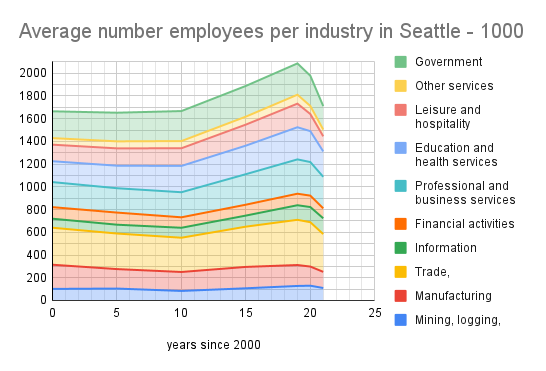
\includegraphics[width=\linewidth]{images/7D79AA67-B877-434A-BE22-808AC2C091B1.png}
                  \caption{stacked chart of $N_{I,C}(t)$ vs $t$ }
                  \label{fig:chart1}
                \end{figure}
                
            As can be seen, the workforce population which is the total height of \ref{fig:chart1} varies with time as expected.
            Plotting $P_{I,C}(t)$ vs $t$ we see: 
            \begin{figure}[H]
                  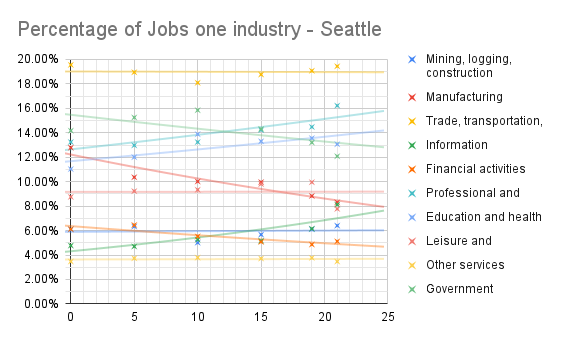
\includegraphics[width=\linewidth]{images/D111796A-6172-47DA-A494-CF6D7A966055.png}
                  \caption{stacked chart of $P_{I,C}(t)$ vs $t$ }
                  \label{fig:chart2}
                \end{figure}
                
                We saw that by Plotting $P_{I,C}(t)$ we see a clearer trend. We also do not need to account for change in population anymore using this method as $P_{I,C}(t)$ is a percentage of the total workforce population. In addition, we removed the data for 2020 as it seemed anomalous for every industry and so we thought it wasn't representative.
                
                
                
            \subsubsection{Exponential model}
            
                % All figures and graphs should have a title, a label, a caption, and the axes should be labelled.
                
                %h (here) – same location
                %t (top) – top of page
                %b (bottom) – bottom of page
                %p (page) – on an extra page
                %! (override) – will force the specified location
                %(\usepackage{float}) allows to set the option to [H], which is even stricter than [h!].
                The next task was to find the function: $P_{I,C}(t)$ in the form:
                \begin{equation}
                P_{I,C}(t) = a \cdot e^{bt}
                \end{equation}
                We are assuming that the proportion of an industry in a city varies as an exponential due to the following reasons: 
                \begin{itemize}
                    \item An exponential model more accurately represent changes in populations and natural growth over time
                    \item An exponential model better fits the data
                    \item An exponential model demonstrates asymptotic behaviour, not allowing for the percentage to fall below a certain level. This is closer to real life as industries will not shrink infinitely to 0. 
                \end{itemize}
                Using exponential regression, we were able to draw an exponential line of best fit for each $P_{I,C}(t)$. 
                
                \subsubsection{The $H_{I}$ constant}
                The Estimated percentage of jobs that can be done at home by occupation category in D3 was the basis for finding a value for $H_{I}$. Although it was not as straight forward as the industries named in D3, were not named the same as the industries in D1, which was the basis for our model of $P_{I,C}(t)$.
                
                So we tried to match each industry in D1 to 1 or more industries in D3. 
                
                We then calculated a value for $H_I$ for every industry in D1 based on the The Estimated percentage of jobs that can be done at home by occupation category in D3. If there are multiple matches we will calculate a weighted average based on the proportion of the certain occupation in the industry for $H_I$.
                
                \begin{tabular}{|p{4.5cm}|c|c|c|} % Defines where vertical lines appear and the column alignment left centre or right
                      \toprule 
                       \textbf{Industry in D1} & \textbf{Industry in D3}  & \textbf{weights} & \textbf{$H_I$}\\
                      \midrule 
                       Mining, logging, construction& Trade, transportation, and utilities & - & 0\%\\
                       Manufacturing& Production & - & 1\%\\
                       Trade, transportation, and utilities& Transportation and material moving & - & 30\%\\
                       Information& Computer and mathematical & - & 100\%\\
                       Financial activities& Business and financial operations & - & 88\%\\
                       Professional and business services & sales-office and administrative-management & 0.5-0.4-0.1 & 49\%\\
                       Education and health services& Education - health services&0.3-0.7 & 34\%\\
                       Leisure and hospitality& Food preparation and service related&- & 0\%\\
                       Other services & - & - & 50\%\\
                       Government & Legal-Office and administrative-Management& 0.2-0.7-0.1 & 74\%\\
                       
                       
                       

                      \bottomrule 
                    \end{tabular}
                
                Health and Education weights sourced from: \cite{eduStats} \cite{eduStats2}.
                
                % (USE THE REF AND LABEL COMMANDS because then figure numbers never go wrong)
                
                

        \subsection{Applying the Model (Results)}  
            % Considering any situations given to us in the question
            % And if none are given, make up some input data into the Model
            As we have 5 cities and 10 industries, we have 50 $P_{I,C}(t)$ functions. In the interest of saving space, I will give one example of this function:
            \begin{align}
            P_{trade,Omaha}(t) &= 0.237e^{-0.0117t} \\
            P_{trade,Omaha}(24) &= 17.90\% \\
            P_{trade,Omaha}(27) &= 17.28\% 
            \end{align}
            \begin{figure}[H]
                  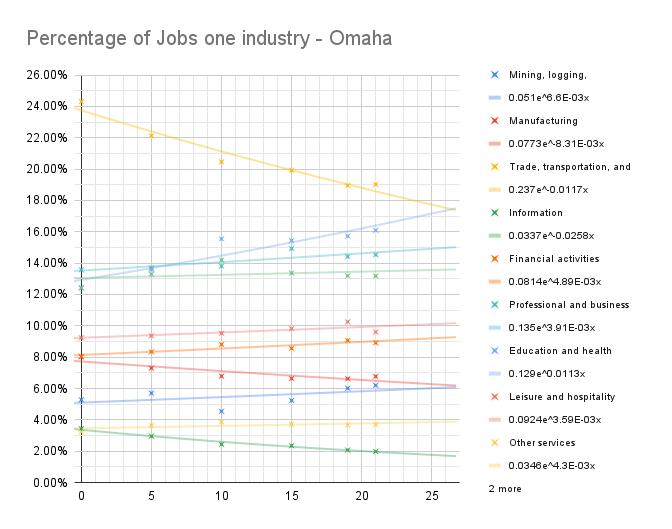
\includegraphics[width=\linewidth]{images/BEAB97A6-07C9-45F9-8B49-E371557909FE.png}
                  \caption{$P_{I,C}(t)$ vs $t$ with exponential trend line}
                  \label{fig:chart3}
                \end{figure}
                
            Finally we can find the percentage of "work from home ready" jobs by multiplying the $P_{I,C}(t)$ function by its corresponding $H_I$ value, and summing the results together to get a percentage of all the "work from home ready" jobs as a proportion of all the jobs in the city: $\Sigma P_{I,C}(t)\cdot H_I$ for all industries in the city.
                
            
            
                 \begin{tabular}{|c|c|c|} % Defines where vertical lines appear and the column alignment left centre or right
                      \toprule 
                       \textbf{City} & \textbf{year 2024}  & \textbf{year 2027} \\
                      \midrule 
                       Seattle & 41.31\% & 41.80\% \\
                       Omaha & 40.22\% & 40.36\% \\
                       Scranton & 35.91\% & 36.16\% \\
                       Liverpool & 31.22\% & 31.04\% \\
                       Barry & 39.07\% & 38.95\% \\
                       
                       
                       

                      \bottomrule 
                    \end{tabular}
                           
            
        \subsection{Implications}
            % What do the results mean?
            Our results show that approximately 40\% of jobs will be "work from home ready". This is not too different from the current rate. This is because we have assumed technology will not change much in the next 5 years to create a considerable change in the proportion of jobs that can be done from home.
            
        \subsection{Evaluating the Model}
            \subsubsection{Validation: Testing for Accuracy}
                % How accurate are the results? Can we use a separate dataset for which we have the "right answer" to check?
                To validate our data we looked online to other predictions for the percentage of jobs that could be done online. one of the pieces of data we came across was a Forbes article \cite{Forbes} that stated that it was about 37\%.And as working from home becomes easier as tech is more integrated into work I would say that our model accurately predicts the proportion of people able to work from home
                
            \subsubsection{Sensitivity Analysis: Testing for Stability and Sensitivity to Assumptions}
                % Sensitivity analysis can be done by taking constants and varying them by +/- n%; use a table for this perhaps.
                % discussion of how the model can be tested for accuracy, stability, and sensitivity to assumptions.
                % Think about what real world factors could lead to changes to a certain parameter value, and then address the effects of those changes on the model.  
                As an example of how sensitive the model is we will use the function $P_{trade,Omaha}(25)$ 
                where $P_{trade,Omaha}(t)&= 0.237e^{-0.0117t}$
                
                \begin{table}[h!]
                  \begin{center}
                    \label{tab:variables1} % Use this to create a label for the table so you can later reference it with \ref
                    \begin{tabular}{|c|c|} % Defines where vertical lines appear and the column alignment left centre or right
                      \toprule 
                       \textbf{$\Delta$ Time} & \textbf{ $P_{trade,Omaha}$} \\
                      \midrule 
                       +5\%  & +0.004\%\\ 
                       -5\% & -0.003\%\\
                      \bottomrule 
                    \end{tabular}
                    \caption{Sensitivity Analysis for Model $P_{trade,Omaha}$} 
                  \end{center}
                \end{table}
            \subsubsection{Model Strengths}
            preserves the impact of decreasing industries\\
            reflects the increasing dominance of certain industries\\
            not sensitive to small changes in time \\
            includes the population of the workforce \\
            uses the changing the pattern of industries in the model\\
        
    
            

            
            \subsubsection{Model Weaknesses}
            Over a very large periods of time (100+years) the model will become unsuitable as there is no way to conceivably predict the market share of each industry.\\
            
